

%\setcounter{chapter}{-1}


\chapter{Множества}

\lesson{1}{08.09.2023}{Операции над множествами}

\section{Операции над множествами}






\begin{notation}
    $x \in A$ означает, что элемент x принадлежит множеству A.
\end{notation}

$x \notin A$ означает, что элемент x не принадлежит множеству A.
    
\begin{definition}
    $\emptyset$, пустое множество - множество, не содержащее ни одного элемента.
\end{definition}



\begin{definition}
    Множество B называют подмножеством A, если любой элемент B принадлежит A.

    \begin{notation}
        $B \subset A$
    \end{notation}

    \begin{eg}
        $\N \subset \Z \subset \Q \subset \R$
    \end{eg}
\end{definition}

Операции.

\begin{enumerate}
    \item Пересечение множеств A и B - это множество из элементов принадлежащих A и B.
    \begin{notation}
        $A \cap B$
    \end{notation}
    \item Объединение множеств A и B - множество из элементов A или B.
    \begin{notation}
        $A \cup B$
    \end{notation}
    \item Разность множеств A и B - множество элементов A, не принадлежащих B.
    \begin{notation}
        $A \setminus B$
    \end{notation}
    \item Симметрическая разность
    \begin{eg}
        $A \triangle B = (A \setminus B) \cup (B \setminus A)$


        $A \triangle B = (A \cup B) \setminus (A \cap B)$
    \end{eg}
    \begin{figure}[H]
        \centering
        \includegraphics[width=\linewidth]{1.png}
        
        
        \label{fig:1}
    \end{figure}
    
    \item Дополнение
    
\end{enumerate}

Если предположить, что все множества являются поднмножествами некоторого универсального множества, дополнение множества A - это множество элементов U, не принадлежащих A.

\begin{figure}[H]
    \centering
    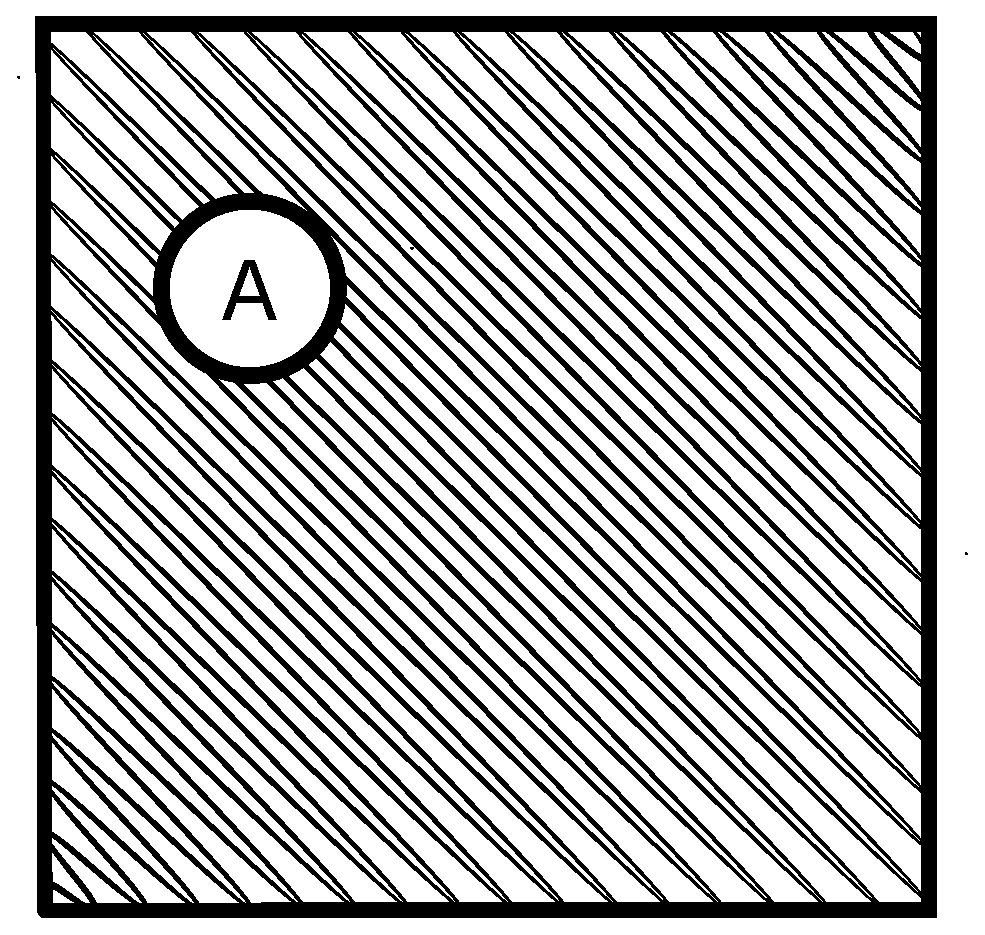
\includegraphics[width=\linewidth]{2.eps}
    
    
    \label{fig:2}
\end{figure}

\begin{eg}
$U = \Z$

$A$ - множество чётных чисел

$\overline A$ - множество нечётных чисел
\end{eg}

Порядок действий
\begin{enumerate}
    \item Дополнение
    \item Пересечение
    \item Объединение, рахность, симметрическая разность
\end{enumerate}
Приоритет слева направо.

\begin{eg}
$U = \{1,2,3,4,5\}$
$A = \{1, 2, 3\}$
$B = \{3, 4\}$
$C = \{4, 5\}$

$\overline{A \cup B \cap \overline{C} \setminus \overline{B}}$
\begin{enumerate}
    \item $\overline{C} = \{1, 2, 3\}$
    \item $\overline{B} = \{1, 2, 5\}$
    \item $B \cap \overline{C} = \{3\}$
    \item $A \cup B \cap \overline{C} = \{1, 2, 3\}$
    \item $A \cup B \cap \overline{C} \setminus \overline{B} = \{3\}$
    \item $\overline{...} = \{1, 2, 4, 5\}$
\end{enumerate}
\end{eg}

Свойства:

\begin{enumerate}
\item {
Дистрибутивность

\begin{enumerate}
    \item $(A \cap B) \cup C = (A \cup C) \cap (B \cup C)$
    \begin{figure}[H]
        \centering
        \includegraphics[width=\linewidth]{3.png}
        
        
        \label{fig:3}
    \end{figure}
    \item $(A \cup B) \cap = (A \cap C) \cup (B \cap C)$
    \begin{figure}[H]
        \centering
        \includegraphics[width=\linewidth]{4.png}
        
        
        \label{fig:4}
    \end{figure}
\end{enumerate}
    

\begin{proof}
Положим $D = (A \cap B) \cup C$

$E = (A \cup C) \cap (B \cup C)$

Докажем, что $C \subset E$

Пусть $x \in D$, тогда выполняется
\begin{enumerate}
    \item $x \in A \cup B$ 
    или
    \item $x \in C$
\end{enumerate}

Если выполнено 1, то x $\in A \cup B => x \in A => x \in A \cup C \in  A \cap B => A \in B => x \in B \cup C => x \in (A \cup C) \cap (B \cup C)$

Если выполнено 2, то $x \in C => x \in A cup C => x \in (A \cup C) \cap (B \cup C)$

$x \in C => x \in B \cup c$

$x \in E => x \in A \cup C$ и $x \in B \cup C$

Случай 1. $x \notin C$

\begin{itemize}
    \item $x \notin C$, $x \in A \cup C => x\in A$
    \item $x \neq C$, $x \in B \cup C => x \in B$
\end{itemize}

$=> x \in A \cap B =. x \in B$

Случай 2. $x \in C$

$=> x \in (A \cap B) \cup C => x \in D$
\end{proof}

}
\item {
Законы де Моргана
\begin{enumerate}
    \item $\overline{A \cup B} = \overline A \cap \overline B$
    \item $\overline{A \cap B} = \overline A \cup \overline B$
\end{enumerate}
}
\end{enumerate}

Прямым или декартовым произведеним множеств A и B называют множество упорядоченных пар
(a, b), где $a \in A$, $b \in B$

\begin{notation}
    $A \times B$
\end{notation}

\begin{eg}
\begin{enumerate}
    \item {
        $A = \{1, 2\}$, $B = \{x, y\}$
    
        $A \times B = \{(1, x), (1, y), (2, x), (2, y)\}$
    }
    \item{
        $A = \{1, 2\}$, $B = \{1\}$

        $A \times B = \{(x, y) | x, y \in \R\}$
    }
    \item {
        $A = B = R$

        $A \times B = \{(x, y) | x, y \in \R\}$
    }
\end{enumerate}
\end{eg}

Св-во: между элементами множеств $(A \times B) \times C$ и $A \times (B \ times C)$ есть взаимно однозначное соответствие.

\begin{definition}
    $A \times B \times C$ - Это $(A \times B) \times C$

    $A^n = A \times A \times ... A$
\end{definition}


\begin{eg}
    ${0, 1}^3$ элементов (0,0,0), (0,0,1), ..., (1,1,1)
\end{eg}


\section{Отображения}

\begin{definition}
    Отображением или функцией из множества X в множество Y называют правило, которое каждому элементу множества X сопоставляет ровно один элемент из множества Y.
\end{definition}

\begin{eg}
\begin{enumerate}
\item {
$X = \{a, b, c, d\}$
$Y = \{1, 2, 3\}$

$f(a) = 1$

$f(b) = 2$

$f(c) = 1$

$f(d) = 1$
}
\item {
$X = Y = \R$

$f(x) = x^2$=
}
\end{enumerate}
\end{eg}


\begin{definition}
    Образом отображения $f$ называют множество элементов $f(x)$ т.к. $\{f(x) | x \in X\}$

    \begin{notation}
        $Imf, f(X)$
    \end{notation}
\end{definition}



\begin{definition}
    Прообразом элемента $y \in X$ называют множество элементов множества X, которые переходят в y, т.е.

    $\{x \in X | f(x) = y\}$

    \begin{figure}[H]
        \centering
        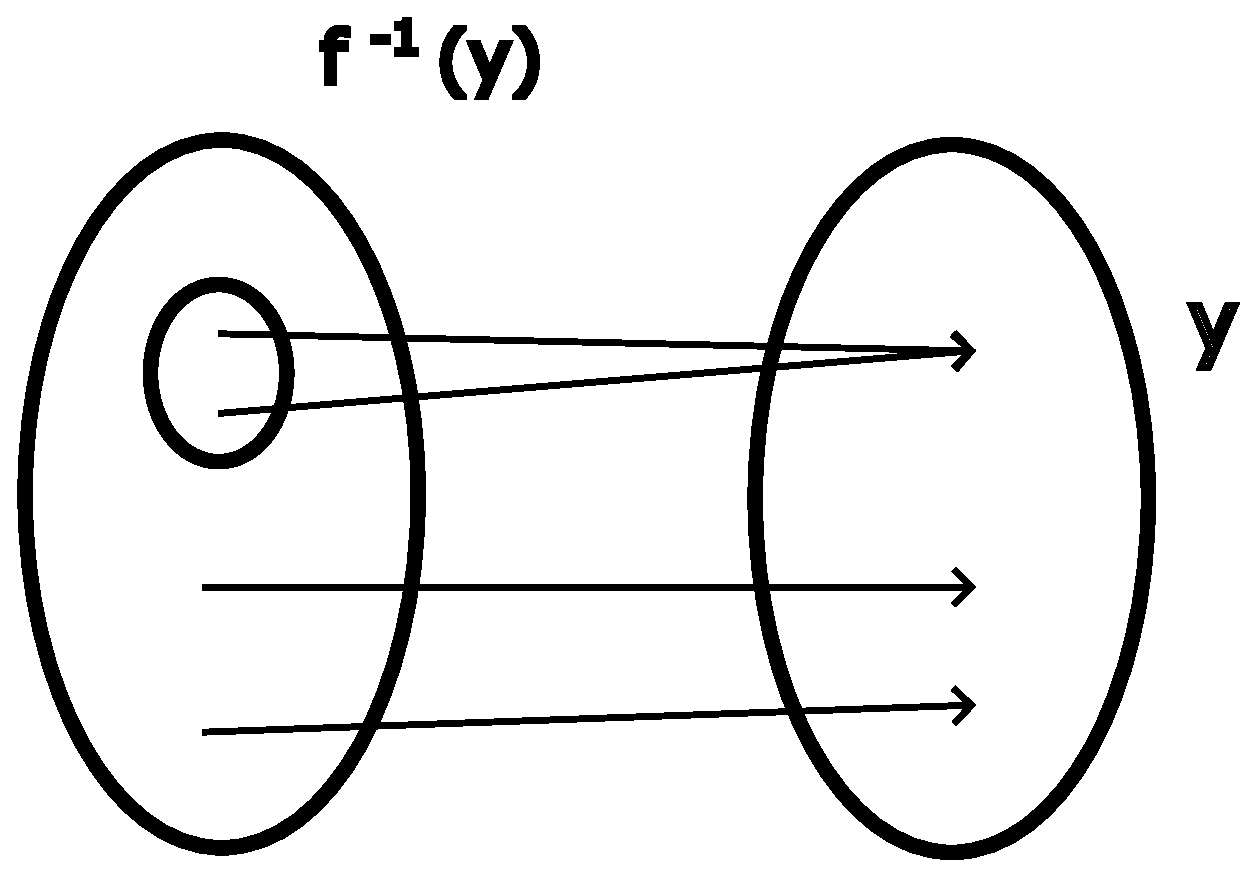
\includegraphics[width=\linewidth]{5.eps}
        
        
        \label{fig:5}
    \end{figure}

    \begin{figure}[H]
        \centering
        \includegraphics[width=\linewidth]{6.png}
        
        
        \label{fig:6}
    \end{figure}

    \begin{notation}
        $f^{-1}(y)$


        Если $y_1 \subset y$, то 


        $f^{-1}(y_1) = \{x \in X | f(x) \in y_1\}$
    \end{notation}
\end{definition}

\begin{definition}
    Отображением $f$ называют иньективным, если прообраз любого элемента содержит не более одного элемента.

    \begin{figure}[H]
        \centering
        \includegraphics[width=\linewidth]{7.png}
        
        
        \label{fig:7}
    \end{figure}

    Др. названия:
    \begin{itemize}
        \item $f$ - иньекция
        \item $f$ является отображением в
    \end{itemize}
\end{definition}

\begin{definition}
    Отображение $f$ называется сюрьективным, если если прообраз любого элемента содержит хотя бы один элемент.

    \begin{figure}[H]
        \centering
        \includegraphics[width=\linewidth]{8.png}
        
        
        \label{fig:8}
    \end{figure}

    Др. названия:
    \begin{itemize}
        \item $f$ - сюрьекция
        \item $f$ является отображением на
    \end{itemize}
\end{definition}

\begin{definition}
    Отображение $f$ называется биективным, если прообраз любого элемента состоит ровно из одного элемента.
    
    Др. названия:
    \begin{itemize}
        \item $f$ - биекция
        \item $f$ - взаимно однозначное отображение
    \end{itemize}
\end{definition}

\begin{remark}
$f$ биекция $<=>$ $f$ - инъекция и сюръекция.
\end{remark}

\begin{eg}
    $f: \Z \rightarrow \Z$
\end{eg}

\begin{enumerate}
    \item $f(x) = x + 1$ - биекция
    \item { $f(x) = x^2$ - не иньекция, не биекция
    
    
    $f^{-1}(4) = \{2. -2\}$


    $f^{-1}(5) = \emptyset$


    $\alpha \subset 2$
    }
    \item {  $f(x) = 2x$ - инъекция, не сюръекция
    
    $f^{-1} = \emptyset$

    $x_1 \neq x_2 => 2x_1 \neq 2x_2$
    }

    \item { $f(x) = [\frac{x}{2}]$ не иньекция
    
    $[\frac{0}{2}] = [\frac{1}{2}]$

    $2n \in f^{-1}(n)$

    => 

    $f^{-1}(n) \neq \emptyset$
    }
\end{enumerate}


\begin{definition}
    Тождественное отображение
    $e_x: x \rightarrow x_1, e_x(x) = x$
\end{definition}

\begin{definition}
    Пусть $y: X - Y, f: X \rightarrow Z$

    \begin{figure}[H]
        \centering
        \includegraphics[width=\linewidth]{9.png}
        
        
        \label{fig:9}
    \end{figure}

    отображение композиция $f o g$ определяется как

    $(f o g)(x) = f(g(x))$

    \begin{eg}
        $X = Y = \Z = \R$

        $f(x) = x + 1, y(x) = x$
        
        $(f o g)(x) = x^2 + 1$
        
        $(g o f)(x) = (x + 1)^2$ 
    \end{eg}

    \begin{remark}
        $(f o g) oh = fo (g o h)$
    \end{remark}

    \begin{notation}
        $f o g o h$
    \end{notation}
\end{definition}

\begin{definition}
    Пусть $f : X \rightarrow Y, y : Y \rightarrow V$

    Отображение y называют образом к отображениб f, если

    

    $f o g = e$ 

    $g o f = e$

    \begin{figure}[H]
        \centering
        \includegraphics[width=\linewidth]{10.png}
        
        
        \label{fig:10}
    \end{figure}

    \begin{figure}[H]
        \centering
        \includegraphics[width=\linewidth]{11.png}
        
        
        \label{fig:11}
    \end{figure}

    \begin{eg}
        $X = Y = [0; +\infty]$

        $f(x) = x^2, y(x) = \sqrt{x}$
    \end{eg}

    \begin{definition}
        Обратное отображение к $f$ обозначается $f^{-1}$

        (Корректность, т.е. единственность отображения обратных - ниже)
    \end{definition}
\end{definition}

\begin{theorem}(Существование обр. отображения)

Обратное отображение к $f$ существует тогда и только тогда, когда $f$ является биекцией.

\begin{proof}
\begin{enumerate}
\item {
Доказать, что если $f$ биекция, то существует $y$, обратное к $f$

Пусть $y \in X \exists! x$, такой, что $f(x) = y$

\begin{figure}[H]
    \centering
    \includegraphics[width=\linewidth]{12.png}
    
    
    \label{fig:12}
\end{figure}

Положим $y(y) = x$

\begin{figure}[H]
    \centering
    \includegraphics[width=\linewidth]{13.png}
    
    
    \label{fig:13}
\end{figure}

$y(f(x)) = g(y) = X$

$=> g o f = e_x$

$f(g(y)) = f(x) = y => f o g = Ry$
}

\item {

Доказать, что если существует $g: g o f = e_x, f o g = e_x$, то $f$ - биекция.

\begin{figure}[H]
    \centering
    \includegraphics[width=\linewidth]{14.png}
    
    
    \label{fig:14}
\end{figure}

\begin{itemize}
\item {
    Иньекция

    Пусть f - не иньекция

    $=> \exists x_1 ... x_2 : f(x_1) = f(x_2)$

    $x_1 = g(f(x_1)) = g(f(x_2)) = x_2$

    Противоречие.
}

\item {
    Сюрьекция

    $f(g(y)) = y => g(y)$ - прообраз $f$
}
\end{itemize}

}
\end{enumerate}
\end{proof}
    
\end{theorem}

\begin{theorem} (Единственности обратного отображения)

    Пусть $f$ - Биекция $X \rightarrow Y$. Тогда не существует различных отображений $y_1, y_2$ являющихся обратными к A.

\begin{proof}
    Доказательство: Упражнение! % TODO: доказать
\end{proof}
\end{theorem}